\vspace{-0.2cm}
\section{Anti-rollover Path Tracking Controller}
\subsection{Mechanism of anti-rollover path tracking}
By utilizing a multi-constraint model predictive control (MPC), the anti-rollover path tracking can explicitly consider input and output constraints. This ensures that, given a reasonably accurate model, as long as a feasible control solution exists, the vehicle will not experience rollover or violate other feasibility constraints. In cases where there is no feasible solution that satisfies all constraints, the solver, aided by relaxation factors, will first violate the least critical soft constraints until it finds a feasible solution with the lowest penalty.

As shown in Fig. \ref{fig:mechanism}, assuming a global reference path has been obtained through cloud-based predictive lane change or other path planning applications, the path tracking controller solves a quadratic programming MPC problem to obtain a feasible control solution sequence that minimizes violations of soft constraints, and selects the first control input from this sequence as the actual control input.

\begin{figure}[!htb]
\centering
\vspace{-0.5cm}
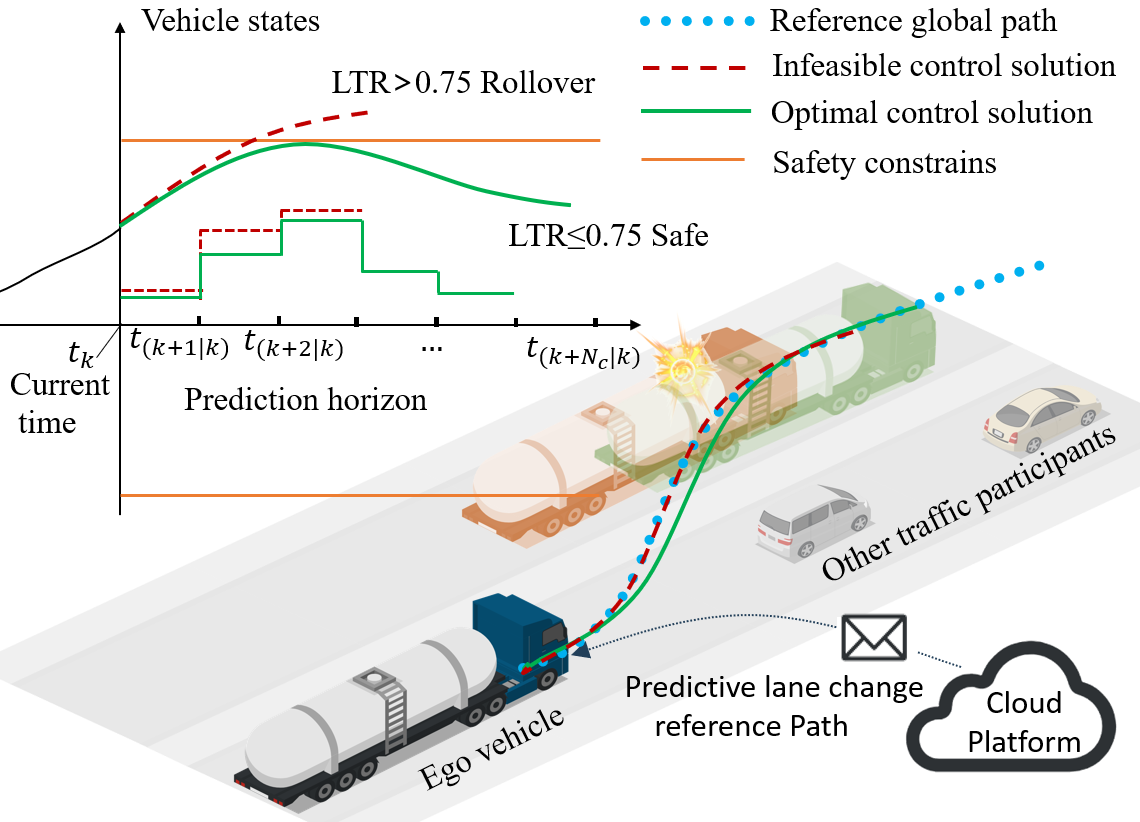
\includegraphics[width=3in]{fig/machanism.png}
\vspace{-0.1cm}
\caption{Mechanism of anti-rollover path tracking based on multi-constrained MPC}
\vspace{-0.5cm}
\label{fig:mechanism}
\end{figure}



\subsection{Optimal control problem construction}
The construction of the optimal control problem in this section includes output design, cost function construction, and constraint design.
The designed outputs are as follows

\vspace{-0.3cm}
\begin{equation}
y = \left[ \theta \,\dot{\theta} \,\psi_1\, Y_1 \,X_1 \,LTR_{eql} \right]^T
\label{eq:yk}
\end{equation}
\vspace{-0.3cm}

Output variables in this study can be divided into three parts:
	 Vehicle attitude for path tracking: $Y_1$, $X_1$, $\psi_1$,
	 linearized equivalent pendulum states for driving sloshing suppression: $\theta$, $\dot{\theta}$,
	 and equivalent load transfer rate based on suspension forces for rollover prevention: $LTR_{eql}$. Even though lateral error is a widely used state variable for tracking \cite{Reviewer1_FuzzySteering}, which makes a linear tracker as shown in Figure.\ref{fig:tracker}, absolute position $Y_1$, $X_1$ are used as the state variables that make an absolute tracker \cite{ShengboEbenLi2024reinforcement} and allow for more accurate prediction of higher-order dynamics in tracking, crucial for managing sloshing and rollover states over a longer prediction horizon up to 1.5 $s$-3 $s$ (covering the sloshing period around 1 $s$\cite{wangZhaoLin2002} to catch potential peaks in $LTR$ dynamics). This approach enhances MPC's effectiveness, ensuring better stability and safety compared to linear trackers that simplify these dynamics.
     
  \vspace{-0.6cm}
\begin{figure}[!hbt]

  \subfloat[]{
    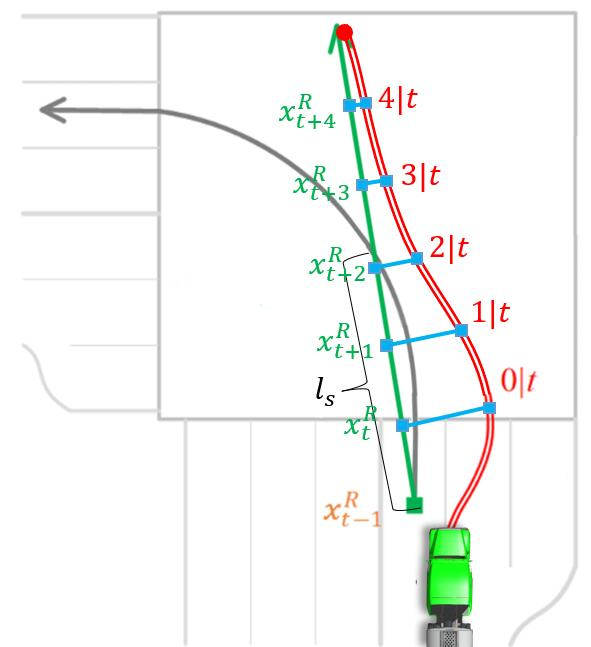
\includegraphics[width=0.215\textwidth]{fig/linear_tracker.jpg}
    \label{fig:linear_tracker}
  }
  \subfloat[]{
    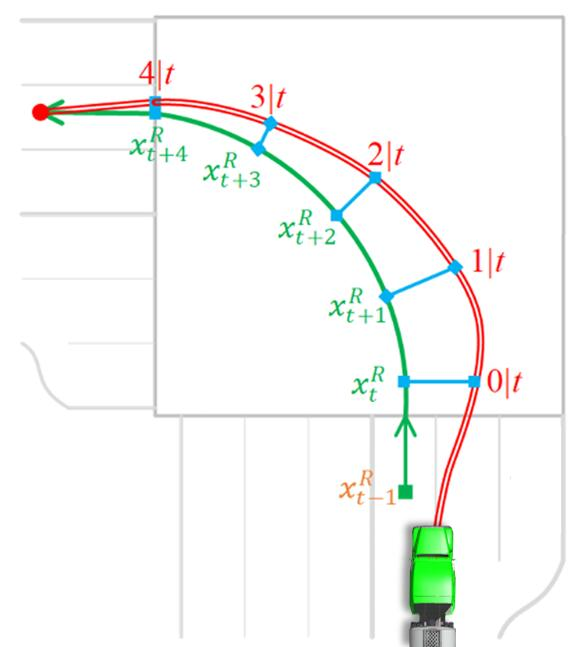
\includegraphics[width=0.21\textwidth]{fig/absolute_tracker.jpg}
    \label{fig:abs_tracker}
  }
  \vspace{-0.1cm}
  
  \caption{Comparison of linear tracker and absolute tracker.(a)Linear tracker (or a tangent tracker when $l_{s} \rightarrow 0$) (b)Absolute tracker. }
  \label{fig:tracker}
  \vspace{-0.3cm}
\end{figure}




The MPC controller in this research corresponds to three functions: path tracking, sloshing suppression, and rollover prevention. For path tracking, only the tractor's state variables are used since the trailer trajectory closely follows the tractor trajectory, making it more convenient in terms of sensor placement and computational complexity. Additionally, forces generated by liquid sloshing depend on both the sloshing angle and angular velocity. Even small changes in the angle can lead to significant lateral forces and roll moments when the angular velocity changes dramatically. Hence, it is necessary to consider both the suppression of liquid sloshing angle and angular velocity. Commonly used indicators for vehicle rollover include static stability factor (SSF), dynamic stability factor (DSF), lateral load transfer rate (LTR), time to rollover (TTR) \cite{MPC_MotionPlanning2021}, zero moment point (ZMP) \cite{ZMP_2017}, and combinations thereof. SSF effectively represents the vehicle's static rollover resistance but lacks suitability for dynamic representation. LTR, TTR, and ZMP better reflect the vehicle's dynamic rollover state and are somewhat equivalent. In this study, LTR is selected as the rollover indicator, although its practical application in engineering is limited due to the difficulty of measuring tire-ground normal force. Consequently, the suspension force equivalent $LTR_{eql}$ is commonly used as a substitute.
\vspace{-0.3cm}
\begin{equation}
LTR_{eql} = c_f \cdot \left( -k_{r1}\phi_1 - c_1 \dot{\phi}_1 - k_{r2}\phi_2 - c_2 \dot{\phi}_2 \right)
\label{eq:LTR_eql}
\end{equation}
\vspace{-0.3cm}
where coefficient $c_f$ is 

\begin{equation}
c_f = \frac{2}{\frac{T_{w1} + T_{w2}}{2} (m_1 + m_2) g}.
\end{equation}

Conditions for $LTR_{eql}\Longleftrightarrow LTR$ are
	 accurate identification of suspension-related parameters ($k_{r1}$, $k_{r2}$, $c_1$, $c_2$), mass parameters ($m_1$, $m_2$), and track widths ($T_{w1}$, $T_{w2}$), and precise measurement or estimation of vehicle roll angle $\phi_i$ and roll angular velocity $\dot{\phi}_i$.

Although achieving these conditions exactly is infeasible in practice, an equivalent value of LTR can still be obtained with high accuracy. $LTR_{eql}$ does not suffer from the ±1 saturation and can accurately reflect the vehicle's rollover dynamics even in extreme situations where one wheel is off the ground. Moreover, the parameters for $LTR_{eql}$ are easily obtainable and computationally efficient. To observe the aforementioned output variables, observation matrix $C_d$ should be defined as
\vspace{-0.2cm}
\begin{equation}
C_{d} = \begin{bmatrix}
\begin{matrix}
0_{5 \times 8} & \mathbf{I}_{5}
\end{matrix} \\
c_{4}
\end{bmatrix}
\end{equation}

where $
\setlength{\arraycolsep}{1.2pt}
c_{4} = c_{f}\begin{bmatrix}
0 & 0 & {- k_{r1}} & {- c_{1}} & 0 & 0 & {- k_{r2}} & {- c_{2}} & 0_{1 \times 6}
\end{bmatrix}\nonumber
$.

The discrete-time model constructed is

\begin{equation}
\left\{
\begin{aligned}
x_{k+1} &= A_d x_k + B_d u_k \\
y_k &= C_d x_k
\end{aligned}
\right.
\end{equation}

The state variable $x_k$ and observation variable $y_k$ are defined in equations (\ref{eq:xk}) and (\ref{eq:yk}), respectively, with the subscripts $k$ omitted. The only control input is the front wheel steering angle $u_k = \delta_k$. 

For path tracking, as shown in Fig. \ref{fig:architecture}, assume that local path planning is provided by predictive cruise control or other applications, the reference values for the vehicle's $Y_{1,k+i}$, $X_{1,k+i}$, $\psi_{1,k+i}$, and $\delta_{k+i}$ are determined according to linear interpolation of the reference path assuming constant speed in the predictive horizon, and a collision-free reference path is assumed. The reference values for $\theta_{r,i}$, $\dot{\theta}_{r,i}$, and $LTR_{eql,r,i}$ are set to 0. 

In this work, to achieve a smoother control effect and enhance the safety of semi - trailer tank trucks, we employed an incremental model predictive control (MPC) approach with output constraints. Specifically, this approach aims to limit the increment of the control input and keep the lateral load transfer ratio at equilibrium ($LTR_{eql}$) within a safe boundary, for example, the interval $[-0.75, 0.75]$. For interested readers seeking a more in - depth understanding of MPC fundamentals, we refer to \cite{BookMPC}.

To accelerate the computational process, we implemented a modified version of the moving block method \cite{Cutler1980DynamicMatrixControl} combined with the constraint set compression (CSC) approach. We defined two compression mapping matrices: $T_{N_p(N_x + N_u)\times N_cN_u}$ and $\Pi_{N_yN_r\times N_p(N_x + N_u)}$. Here, $N_p$ represents the prediction horizon, $N_x$ is the number of state variables, $N_u$ is the number of control inputs, $N_c$ is the number of decision variables, and $N_r$ is the number of constrained steps within the prediction horizon, with the conditions $N_c, N_r \leq N_p$. By reducing the number of decision variables and output constraints for time steps farther from the current one within the prediction horizon, we can significantly reduce the peak solving time of the quadratic programming (QP) problem, especially when the active set is large. According to \cite{EbenLi_FastMPC}, this approach has less than a 1\% impact on the optimality of the control solutions. These measures are crucial for the real - time control of semi - trailer tank trucks with high - dimensional state spaces.

To handle potential conflicts between input and output hard constraints and apply soft constraints to output variables, we introduced a relaxation term $\rho\epsilon^2$ into the cost function $J$. Here, $\epsilon$ is the relaxation factor, and $\rho$ is the relaxation coefficient \cite{soft_constraint_Eben2010}. 

In highly uncertain situations, to guarantee robust stability, we tightened the output constraints to ensure that the vehicle state remains within the stability domain. This approach is similar to the dual - mode MPC \cite{soft_constraint_Eben2010}. However, unlike dual - mode MPC, we do not switch the controller strategy for asymptotic stability, as this is not feasible for real - world tracking problems. Instead, we ensure Lyapunov stability within the stability domain.

The MPC problem is reformulated as a standard quadratic programming (QP) problem as shown below:
 
\vspace{-0.1cm}
\begin{equation}
\begin{matrix}
{\underset{\Delta U}{argmin}{J = \frac{1}{2}\begin{bmatrix}
{\Delta U^{T}} & \epsilon
\end{bmatrix}\begin{bmatrix}
H & 0 \\
0 & \rho
\end{bmatrix}\begin{bmatrix}
{\Delta U} \\
\epsilon
\end{bmatrix} + \begin{bmatrix}
g^{T} & 0
\end{bmatrix}\begin{bmatrix}
{\Delta U} \\
\epsilon
\end{bmatrix}}} \\
{s.t.\left\{ \begin{matrix}
{A_{t}\Delta U \leq U_{max} - U_{t}} \\
{{- A}_{t}\Delta U \leq U_{min} + U_{t}} \\
{\Pi\Theta T\Delta U - \epsilon \leq \Pi\left( Y_{max} - E \right)} \\
{- \Pi\Theta T\Delta U - \epsilon \leq \Pi\left( Y_{min} - E \right)} \\
{\Delta U_{min} \leq \Delta U \leq \Delta U_{max}} \\
{\epsilon_{min} \leq \epsilon \leq \epsilon_{max}}
\end{matrix} \right.}
\end{matrix}
\end{equation}

The constructed cost function is in a standard quadratic form, which can be efficiently solved using various QP solvers, such as osqp, qpOASES, and CVXOPT. In this study, we selected qpOASES to solve the QP problems.








